\documentclass[aspectratio=169]{beamer}
\usetheme{Warsaw}
\usepackage[utf8]{inputenc}
\usepackage[english]{babel}
\usepackage{amsmath}
\usepackage{amsfonts}
\usepackage{amssymb}
\usepackage{graphicx}
\usepackage{tikz}
\usetikzlibrary{
	arrows,
	automata,
        shadings,
        shadows,
        shapes,
}

\usepackage{pgfplots}
\usepackage{fontspec}
\newfontfamily\cjkfont{Noto Sans CJK SC} % Or any appropriate font you have

%\usepackage[dvipsnames]{xcolor}
\usepackage{xcolor}

%%  -------------------------------------------------------------------
%%      GDS II layer, regarding MOSIS SCMOS layer map
%%  -------------------------------------------------------------------
% GDS II #41 - P_WELL
\definecolor{pwell}{rgb}{1.0, 0.74, 0.53}   % macaroni and cheese
% GDS II #42 - N_WELL
\definecolor{nwell}{rgb}{0.61, 0.87, 1.0}  % columbia blue
\definecolor{pbase}{rgb}{1.0, 0.51, 0.26}  % mango tango
\definecolor{nbase}{rgb}{0.0, 0.75, 1.0}   % capri 
% GDS II #43 - ACITVE
\definecolor{active}{rgb}{0.9, 0.4, 0.38}   % light carmine pink
% GDS II #45 - N_PLUS_SELECT
\definecolor{nimplant}{rgb}{0.45, 0.76, 0.983}% maya blue
% GDS II #44 - P_PLUS_SELECT
\definecolor{pimplant}{rgb}{1.0, 0.51, 0.26}% mango tango
% GDS II #46 - POLY
\definecolor{poly}{rgb}{0.56, 0.93, 0.56}   % light green
% GDS II #25 - CONTACT
\definecolor{contact}{rgb}{0.83, 0.83, 0.83}% light gray
% GDS II #49 - METAL1
\definecolor{metal1}{rgb}{0.38, 0.31, 0.86} % majorelle blue
% GDS II #50 - VIA1
\definecolor{via1}{rgb}{0.83, 0.83, 0.83}   % light gray
% GDS II #51 - METAL2
\definecolor{metal2}{rgb}{0.04, 0.85, 0.32} % malachite
% GDS II #61 - VIA2
\definecolor{via2}{rgb}{0.83, 0.83, 0.83}   % light gray
% GDS II #63 - METAL3
\definecolor{metal3}{rgb}{0.98, 0.93, 0.37} % maize
% GDS II #30 - VIA3
\definecolor{via3}{rgb}{0.83, 0.83, 0.83}   % light gray
% GDS II #31 - METAL4
\definecolor{metal4}{rgb}{0.75, 0.25, 0.0}  % mahogany
% GDS II #32 - VIA4
\definecolor{via4}{rgb}{0.83, 0.83, 0.83}   % light gray
% GDS II #33 - METAL5
\definecolor{metal5}{rgb}{0.79, 0.08, 0.48} % magenta (dye)
% GDS II #36 - VIA5
\definecolor{via5}{rgb}{0.83, 0.83, 0.83}   % light gray
% GDS II #37 - METAL6
\definecolor{metal6}{rgb}{0.11, 0.35, 0.02} % lincoln green
% GDS II #29 - SILICIDE_BLOCK
\definecolor{silicide-block}{rgb}{0.98, 0.94, 0.9}  % linen
% GDS II #52 - GLASS
\definecolor{glass}{rgb}{1.0, 1.0, 0.88}    % light yellow
% GDS II #26 - PADS
\definecolor{pads}{rgb}{0.75, 1.0, 0.0}     % lime (color wheel)

\definecolor{resist}{rgb}{0.71, 0.4, 0.11}  % light brown

\definecolor{silicide}{rgb}{0.29, 0.33, 0.13}
\definecolor{titanium}{rgb}{0.8, 0.58, 0.46}

\def\OpacityLayout {0.5}

%
% physical
%
\definecolor{substrate}{rgb}{0.96, 0.94, 0.93}  % isabelline
\definecolor{nitride}{rgb}{1.0, 0.03, 0.0}
\definecolor{gateoxide}{rgb}{0.88, 1.0, 1.0}    % light cyan
\definecolor{isolationoxide}{rgb}{0.84, 0.79, 0.87}% languid lavender

\def\CrossSectionOnly{0.3}
\def\CrossAndTopSection{0.2}
\def\CrossAndTopSectionBig{0.3}
\def\VLSILayout{0.4}
\def\UpperContactResist{8.0}
\def\UpperMetalResist{9.0}
\def\UpperMoreMetalResist{16.0}

\def\LowerMetal{4.0}
\def\UpperMetal{4.5}

\def\LowerMoreMetal{5.0}
\def\UpperMoreMetal{5.5}

\def\LowerMoreMetalTwo{6.0}
\def\UpperMoreMetalTwo{6.5}

\def\UpperGlass{7.0}


\author{leviathanch | chipforge | foshardware \ (Lanceville Technology)}
\title{Breaking the microchip monopoly}
\setbeamercovered{transparent} 
\setbeamertemplate{navigation symbols}{} 
%\institute{} 
%\date{} 
\subject{A free semiconductor manufacturing standard}
\begin{document}

%\begin{frame}
%\tableofcontents
%\end{frame}

\section[Standard Cells]{}
\begin{frame}{Standard Cells}
\end{frame}

\section[Silicon Compiler]{}
\begin{frame}{Open Source Tools}
	\begin{itemize}
        \setlength\itemsep{1em}
		\item yosys
		\item graywolf
		\item qrouter
		\item several FPGA routers
	\end{itemize}
\end{frame}

\begin{frame}{graywolf}
	\begin{itemize}
        \setlength\itemsep{1em}
		\item Originates in Academia: TimberWolf
		\item Simulated annealing
	        \begin{itemize}
		    \item Meta heuristic that is useful not only for placement
	        \end{itemize}
		\item Inline syscalls
	        \begin{itemize}
		    \item This is just a bad idea
	        \end{itemize}
	\end{itemize}
\end{frame}

\begin{frame}{qrouter}
	\begin{itemize}
        \setlength\itemsep{1em}
		\item Started in 2011 by Tim Edwards 
		\item Widely used for FPGA
	        \begin{itemize}
		    \item Not ready for silicon
	        \end{itemize}
		\item Sequential routing
	        \begin{itemize}
		    \item Parallelism not in scope
	        \end{itemize}
		\item Difficult to prove formal correctness
	        \begin{itemize}
		    \item Prove that C implementation of Rip-up and Re-route is correct
	        \end{itemize}
	\end{itemize}
\end{frame}

\begin{frame}{Productive Tools}
	\begin{itemize}
        \setlength\itemsep{1em}
		\item Different tool sets like BonnRoute, Cadence Suite, Alliance tools, etc.
		\item Similar capabilities with respect to silicon
		\item Just throw man-power at VLSI --- what is automation?
	\end{itemize}
\end{frame}

{
\setbeamercolor{background canvas}{bg=black}
\begin{frame}
    \begin{center}
        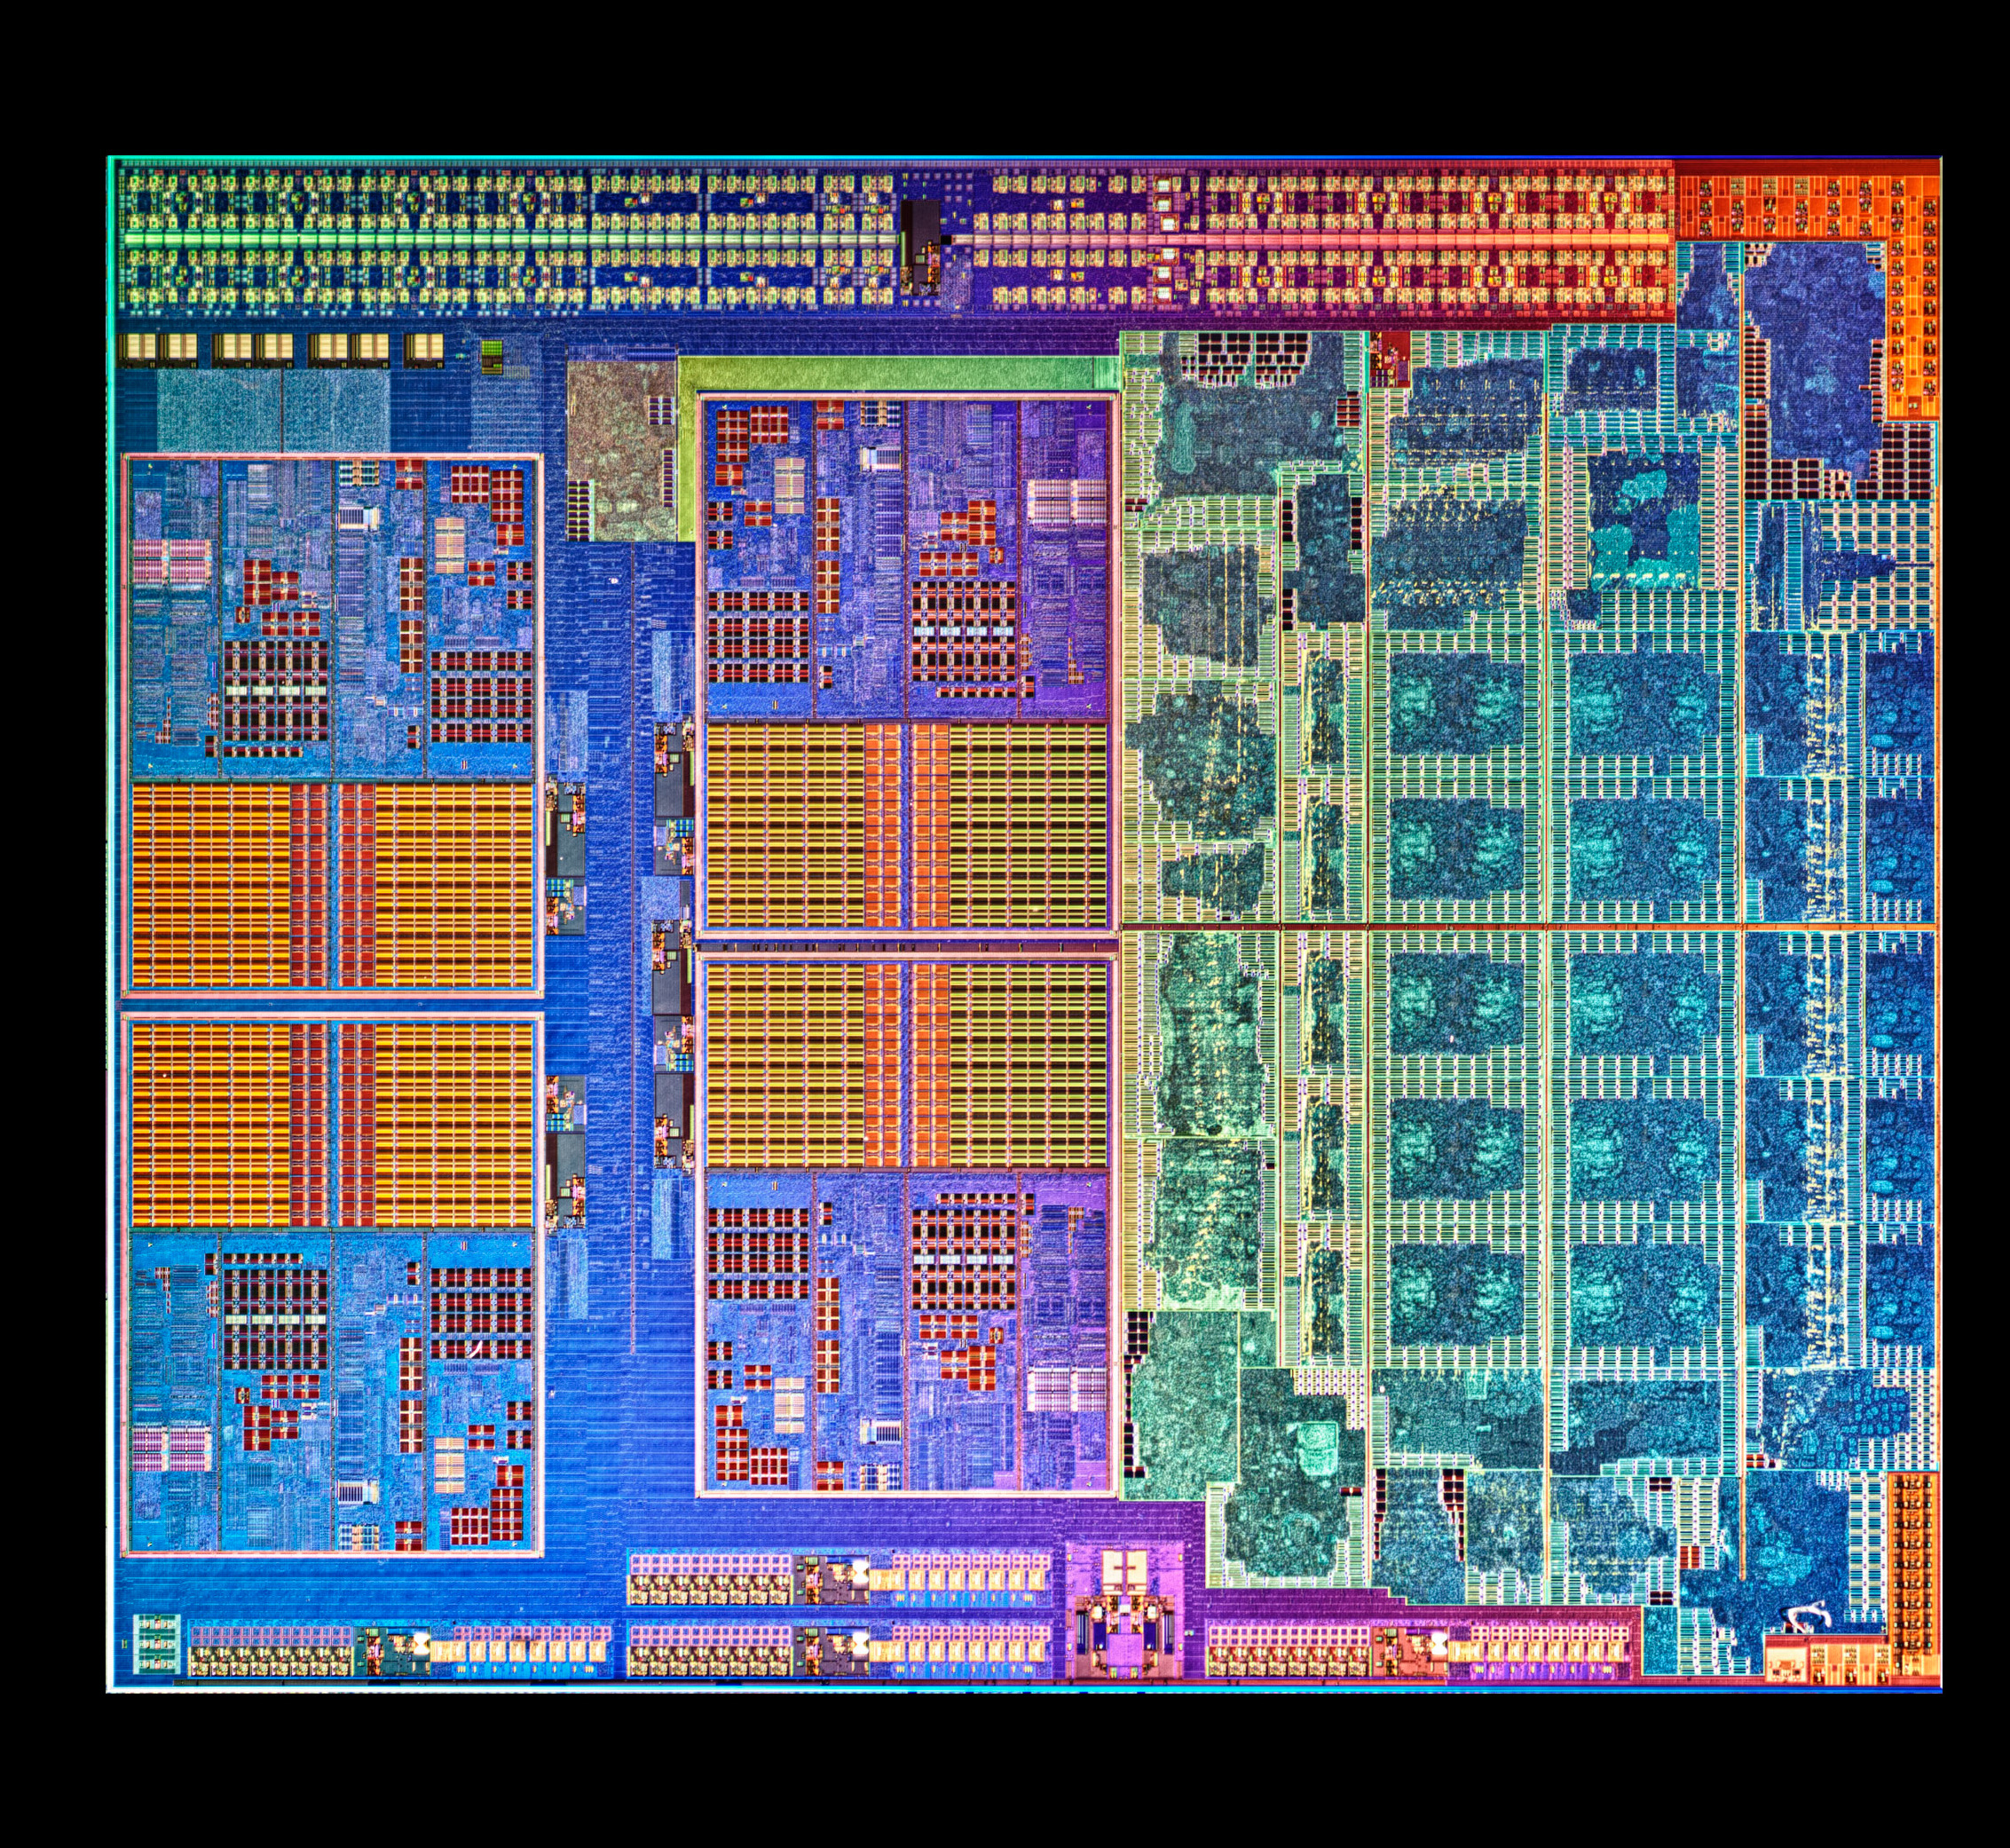
\includegraphics[height=\textheight]{images/VLSI01_rotated.jpg}
    \end{center}
\end{frame} 
}

\begin{frame}{Routing: State of the Art}
	\begin{itemize}
        \setlength\itemsep{1em}
		\item Place components for a large chip
		\item Route wires roughly along a chessboard for a large chip
		\item Route detailed tracks and vias for a large chip
		\item Formal correctness: Rip-up and Re-route
		\item Formal style: Sequential/Imperative code
	\end{itemize}
\end{frame}

\begin{frame}{Routing: Proposed}
	\begin{itemize}
        \setlength\itemsep{1em}
		\item Decomposition for a large chip
		\item Place components and route for small chips in parallel
		\item Place abstract gates and route recursively
		\item Formal correctness: Reduction from SMT
		\item Formal style: Parallel/Declarative code
	\end{itemize}
\end{frame}

\begin{frame}{Divide and Conquer}
	    \textbf{Academia + Industry:}
	    \begin{itemize}
		\item Placement and Routing are different problems
		\item All components map to the same problem
	    \end{itemize}
	    \textbf{LibreSilicon:}
	    \begin{itemize}
		\item Placement and Routing are the same problem
		\item Different components map to different problems
	    \end{itemize}
\end{frame}

\begin{frame}{Routing Hierarchy}
	    \textbf{Academia + Industry:}
	    \begin{itemize}
		\item Geographical partitioning of a wafer $\rightarrow$ \textit{cut tree}
		\item Based on preceeding placement steps
	    \end{itemize}
	    \textbf{LibreSilicon:}
	    \begin{itemize}
		\item Modular chip development $\rightarrow$ \textit{subcell hierarchy}
		\item Subcells carry implicit and explicit subcells
	    \end{itemize}
\end{frame}

\begin{frame}{Frontier: Parallelism}
	\begin{itemize}
        \setlength\itemsep{1em}
		\item BonnRoute: concurrency + shared memory model
		\item qrouter: none 
		\item lsc: map + reduce
	\end{itemize}
\end{frame}

\begin{frame}{Subcell hierarchies}
	\begin{itemize}
        \setlength\itemsep{1em}
		\item Explicit subcell hierarchies through high modularization
		\item Implicit subcell hierarchies through exlining
		\item Preserve hierarchy in compiler interfaces
	\end{itemize}
\end{frame}

\begin{frame}{High modularization}
        \begin{figure}
        \centering
        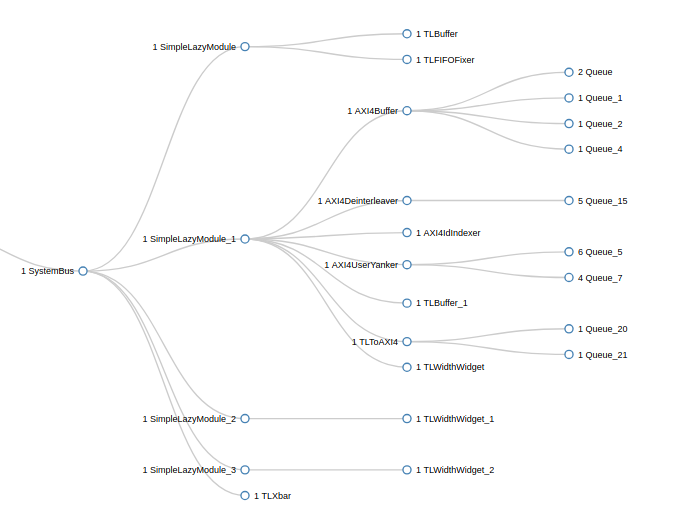
\includegraphics[scale=0.42]{images/SystemBus.png}
        \end{figure}
        \begin{center}
            \href{url}{\scalebox{0.5}{https://murmur.libresilicon.com/lsc/rocket-chip-yosys}}
        \end{center}
\end{frame}

\begin{frame}{Exlining}
	\begin{itemize}
        \setlength\itemsep{1em}
		\item Proof of concept: picorv
	\end{itemize}
        \begin{center}
            \href{url}{\scalebox{0.5}{https://murmur.libresilicon.com/lsc/rocket-chip-exline}}
        \end{center}
\end{frame}

\begin{frame}{Unconstrained Small Unified Silicon Problem}
	\begin{itemize}
        \setlength\itemsep{1em}
		\item Components and nets $\rightarrow$ \textit{rectilinear geometries}
		\item Components do not overlap
		\item Nets overlap with their pins on components
	\end{itemize}
\end{frame}

\begin{frame}{Minimizing Goals}
	\begin{itemize}
        \setlength\itemsep{1em}
		\item Layout area
		\item Maximum wire length 
		\item Via count
		\item Crossing number (computational)
		\item Wire jogs (minor)
	\end{itemize}
\end{frame}

\begin{frame}{Satisfiability Modulo Theories}
	\begin{itemize}
        \setlength\itemsep{1em}
            \item Optimization problems
            \item Abstraction from Boolean satisfiability
            \item Several solvers implement smtlib2
	    \begin{itemize}
                \item \textit{ABC} from University of Berkeley
                \item \textit{CVC4} from Stanford
                \item \textit{Boolector} from Johannes Kepler University
                \item \textit{MathSAT} from Fondazione Bruno Kessler and DISI-University of Trento
                \item \textit{Yices} from SRI
                \item \textit{Z3} from Microsoft
	    \end{itemize}
	\end{itemize}
\end{frame}

\begin{frame}{Boolean Satisfiability}
    \begin{center}
        $ ( \alpha_{1} \vee \alpha_{2} \vee \alpha_{3} )
    \land ( \neg \alpha_{4} \vee \alpha_{5} \vee \alpha_{6} )
        $
    \end{center}
\end{frame}

\begin{frame}{Defining rectangular components}
	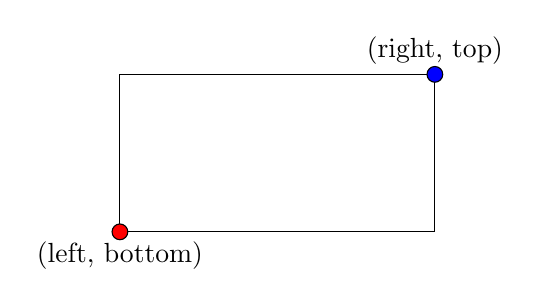
\begin{tikzpicture}
            \draw (0,-8) rectangle (4,-6);
            \draw[fill=red]  (0,-8) circle (0.1);
            \draw[fill=blue] (4,-6) circle (0.1);
            \node at (0,-8.3) {(left, bottom)};
            \node at (4,-5.7) {(right, top)};
	\end{tikzpicture}
\end{frame}

\begin{frame}{Overlaps}
	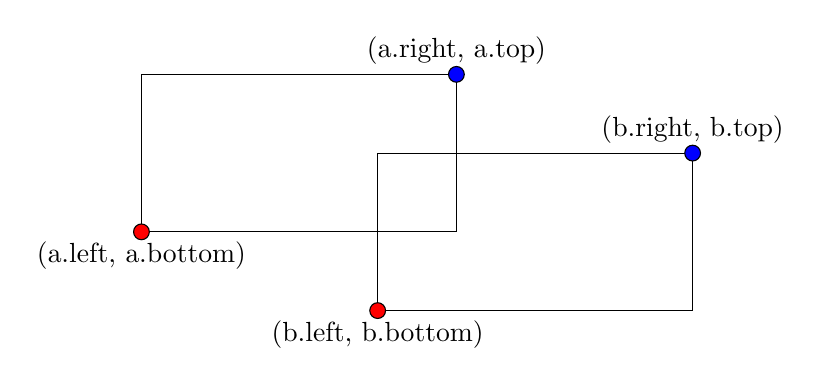
\begin{tikzpicture}
            \draw (0,-8) rectangle (4,-6);
            \draw[fill=red]  (0,-8) circle (0.1);
            \draw[fill=blue] (4,-6) circle (0.1);
            \node at (0,-8.3) {(a.left, a.bottom)};
            \node at (4,-5.7) {(a.right, a.top)};
            
            \draw (3,-9) rectangle (7,-7);
            \draw[fill=red]  (3,-9) circle (0.1);
            \draw[fill=blue] (7,-7) circle (0.1);
            \node at (3,-9.3) {(b.left, b.bottom)};
            \node at (7,-6.7) {(b.right, b.top)};
	\end{tikzpicture}
\end{frame}

\begin{frame}{Reduction from SMT}
        b.left > a.right
    $\parallel$ a.bottom > b.top
\end{frame}

\begin{frame}{Combining in the LSC Semigroup}
    \begin{center}
        overlap + net connect + another constraint
    \end{center}
\end{frame}

\begin{frame}{Stay low}
    \begin{tikzpicture}
        \begin{axis}
          [ xticklabels={,,}
          , yticklabels={,,}
          , scaled ticks=false
          , xmin=0,ymin=0
          , samples=123
          , domain=0:42
          , width=1.1\textwidth,
          , height=0.55\textwidth
          ]
        \addplot[blue] {pow(2,x)} node[above]{};
        \end{axis}
    \end{tikzpicture}
\end{frame}

\begin{frame}{Maximize yield}
	\begin{itemize}
        \setlength\itemsep{1em}
		\item Minimize area of a chip $\rightarrow$ \textit{silicon compiler}
		\item Minimize physical errors $\rightarrow$ \textbf{silicon process}
	\end{itemize}
\end{frame}


\section[Process]{}

\begin{frame}{Features}
	\begin{itemize}
        \setlength\itemsep{1em}
		\item MOSFETs
		\item LDMOSFETs (High voltage) 
		\item BJTs
		\item Zener polysilicon diodes
		\item SONOS flash cells
		\item Polysilicon resistors
		\item Metal caps
	\end{itemize}
\end{frame}

\begin{frame}{Process design considerations}
	\begin{itemize}
		\item Should be portable
		\item Robust
		\item Low amount of layers
		\item KISS (Keep it simple and stupid)
		\item Avoid expensive machines (can be manufactured in a home lab)
	\end{itemize}
\end{frame}

\begin{frame}{Process design considerations}
\begin{center}
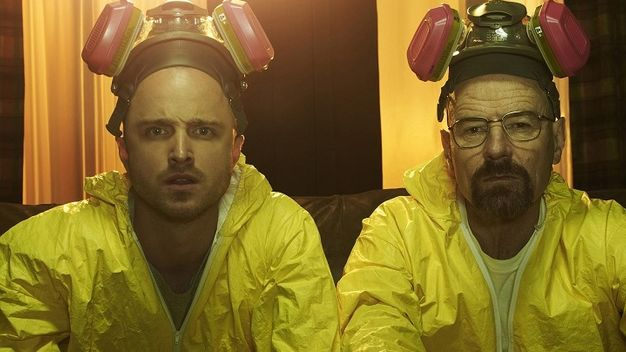
\includegraphics[height=0.8\textheight]{images/breaking-bad.jpg}
\end{center}
\end{frame}

\begin{frame}{Process design considerations}
\begin{center}

\includegraphics[height=0.8\textheight]{images/innovation-hub-hamburg.jpg}
\end{center}
\end{frame}


\begin{frame}{Cross section}
\begin{center}
	\begin{tikzpicture}[node distance = 3cm, auto, thick,scale=0.2, every node/.style={transform shape}]
		\fill[isolationoxide] (0.0,\LowerMoreMetalTwo) rectangle (55.0,\UpperGlass);

\fill[isolationoxide] (0.0,\LowerMoreMetal) rectangle (55.0,\LowerMoreMetalTwo);

\input{tikz_process_steps/more_metal.a.tex}

\fill[white] (2.75,\UpperMoreMetal) rectangle (4.25,\LowerMoreMetalTwo);
\fill[white] (5.50,\UpperMoreMetal) rectangle (7.0,\LowerMoreMetalTwo);
\fill[white] (8.25,\UpperMoreMetal) rectangle (9.75,\LowerMoreMetalTwo);
\fill[white] (11.00,\UpperMoreMetal) rectangle (12.5,\LowerMoreMetalTwo);
\fill[white] (13.75,\UpperMoreMetal) rectangle (15.25,\LowerMoreMetalTwo);

\fill[white] (20.35,\UpperMoreMetal) rectangle (21.65,\LowerMoreMetalTwo);
\fill[white] (22.60,\UpperMoreMetal) rectangle (23.90,\LowerMoreMetalTwo);
\fill[white] (24.35,\UpperMoreMetal) rectangle (25.65,\LowerMoreMetalTwo);

\fill[white] (26.35,\UpperMoreMetal) rectangle (27.65,\LowerMoreMetalTwo);
\fill[white] (28.10,\UpperMoreMetal) rectangle (29.15,\LowerMoreMetalTwo);
\fill[white] (29.60,\UpperMoreMetal) rectangle (30.65,\LowerMoreMetalTwo);
\fill[white] (31.10,\UpperMoreMetal) rectangle (32.15,\LowerMoreMetalTwo);
\fill[white] (32.60,\UpperMoreMetal) rectangle (33.90,\LowerMoreMetalTwo);

\fill[white] (35.10,\UpperMoreMetal) rectangle (36.15,\LowerMoreMetalTwo);
\fill[white] (36.85,\UpperMoreMetal) rectangle (37.90,\LowerMoreMetalTwo);
\fill[white] (38.35,\UpperMoreMetal) rectangle (39.40,\LowerMoreMetalTwo);
\fill[white] (39.85,\UpperMoreMetal) rectangle (40.90,\LowerMoreMetalTwo);
\fill[white] (41.15,\UpperMoreMetal) rectangle (42.15,\LowerMoreMetalTwo);

\fill[white] (43.0,\UpperMoreMetal) rectangle (44.5,\LowerMoreMetalTwo);
\fill[white] (46.5,\UpperMoreMetal) rectangle (48.0,\LowerMoreMetalTwo);

\fill[white] (48.75,\UpperMoreMetal) rectangle (50.25,\LowerMoreMetalTwo);
\fill[white] (52.75,\UpperMoreMetal) rectangle (54.25,\LowerMoreMetalTwo);


\fill[metal3] (2.75,\UpperMoreMetal) rectangle (4.25,\LowerMoreMetalTwo);
\fill[metal3] (5.50,\UpperMoreMetal) rectangle (7.0,\LowerMoreMetalTwo);
\fill[metal3] (8.25,\UpperMoreMetal) rectangle (9.75,\LowerMoreMetalTwo);
\fill[metal3] (11.00,\UpperMoreMetal) rectangle (12.5,\LowerMoreMetalTwo);
\fill[metal3] (13.75,\UpperMoreMetal) rectangle (15.25,\LowerMoreMetalTwo);

\fill[metal3] (20.35,\UpperMoreMetal) rectangle (21.65,\LowerMoreMetalTwo);
\fill[metal3] (22.60,\UpperMoreMetal) rectangle (23.90,\LowerMoreMetalTwo);
\fill[metal3] (24.35,\UpperMoreMetal) rectangle (25.65,\LowerMoreMetalTwo);

\fill[metal3] (26.35,\UpperMoreMetal) rectangle (27.65,\LowerMoreMetalTwo);
\fill[metal3] (28.10,\UpperMoreMetal) rectangle (29.15,\LowerMoreMetalTwo);
\fill[metal3] (29.60,\UpperMoreMetal) rectangle (30.65,\LowerMoreMetalTwo);
\fill[metal3] (31.10,\UpperMoreMetal) rectangle (32.15,\LowerMoreMetalTwo);
\fill[metal3] (32.60,\UpperMoreMetal) rectangle (33.90,\LowerMoreMetalTwo);

\fill[metal3] (35.10,\UpperMoreMetal) rectangle (36.15,\LowerMoreMetalTwo);
\fill[metal3] (36.85,\UpperMoreMetal) rectangle (37.90,\LowerMoreMetalTwo);
\fill[metal3] (38.35,\UpperMoreMetal) rectangle (39.40,\LowerMoreMetalTwo);
\fill[metal3] (39.85,\UpperMoreMetal) rectangle (40.90,\LowerMoreMetalTwo);
\fill[metal3] (41.15,\UpperMoreMetal) rectangle (42.15,\LowerMoreMetalTwo);

\fill[metal3] (43.0,\UpperMoreMetal) rectangle (44.5,\LowerMoreMetalTwo);
\fill[metal3] (46.5,\UpperMoreMetal) rectangle (48.0,\LowerMoreMetalTwo);

\fill[metal3] (48.75,\UpperMoreMetal) rectangle (50.25,\LowerMoreMetalTwo);
\fill[metal3] (52.75,\UpperMoreMetal) rectangle (54.25,\LowerMoreMetalTwo);

% wire
\fill[metal3] ( 2.50,\LowerMoreMetalTwo) rectangle ( 4.50,\UpperMoreMetalTwo);
\fill[metal3] ( 5.25,\LowerMoreMetalTwo) rectangle ( 7.25,\UpperMoreMetalTwo);
\fill[metal3] ( 8.00,\LowerMoreMetalTwo) rectangle (10.00,\UpperMoreMetalTwo);
\fill[metal3] (10.75,\LowerMoreMetalTwo) rectangle (12.75,\UpperMoreMetalTwo);
\fill[metal3] (13.50,\LowerMoreMetalTwo) rectangle (15.50,\UpperMoreMetalTwo);

\fill[metal3] (20.00,\LowerMoreMetalTwo) rectangle (22.00,\UpperMoreMetalTwo);
\fill[metal3] (22.50,\LowerMoreMetalTwo) rectangle (24.00,\UpperMoreMetalTwo);
\fill[metal3] (24.25,\LowerMoreMetalTwo) rectangle (25.75,\UpperMoreMetalTwo);

\fill[metal3] (26.15,\LowerMoreMetalTwo) rectangle (27.75,\UpperMoreMetalTwo);
\fill[metal3] (28.00,\LowerMoreMetalTwo) rectangle (29.25,\UpperMoreMetalTwo);
\fill[metal3] (29.50,\LowerMoreMetalTwo) rectangle (30.75,\UpperMoreMetalTwo);
\fill[metal3] (30.95,\LowerMoreMetalTwo) rectangle (32.30,\UpperMoreMetalTwo);
\fill[metal3] (32.50,\LowerMoreMetalTwo) rectangle (34.25,\UpperMoreMetalTwo);

\fill[metal3] (34.75,\LowerMoreMetalTwo) rectangle (36.25,\UpperMoreMetalTwo);
\fill[metal3] (36.50,\LowerMoreMetalTwo) rectangle (38.00,\UpperMoreMetalTwo);
\fill[metal3] (38.25,\LowerMoreMetalTwo) rectangle (39.50,\UpperMoreMetalTwo);
\fill[metal3] (39.75,\LowerMoreMetalTwo) rectangle (40.95,\UpperMoreMetalTwo);
\fill[metal3] (41.10,\LowerMoreMetalTwo) rectangle (42.35,\UpperMoreMetalTwo);

\fill[metal3] (42.75,\LowerMoreMetalTwo) rectangle (44.75,\UpperMoreMetalTwo);
\fill[metal3] (46.25,\LowerMoreMetalTwo) rectangle (48.25,\UpperMoreMetalTwo);

\fill[metal3] (48.50,\LowerMoreMetalTwo) rectangle (50.50,\UpperMoreMetalTwo);
\fill[metal3] (52.50,\LowerMoreMetalTwo) rectangle (54.50,\UpperMoreMetalTwo);



\fill[white] ( 2.65,\UpperMoreMetalTwo) rectangle ( 4.35,\UpperGlass);
\fill[white] ( 5.35,\UpperMoreMetalTwo) rectangle ( 7.15,\UpperGlass);
\fill[white] ( 8.10,\UpperMoreMetalTwo) rectangle ( 9.90,\UpperGlass);
\fill[white] (10.85,\UpperMoreMetalTwo) rectangle (12.65,\UpperGlass);
\fill[white] (13.60,\UpperMoreMetalTwo) rectangle (15.40,\UpperGlass);

\fill[white] (20.10,\UpperMoreMetalTwo) rectangle (21.90,\UpperGlass);
\fill[white] (22.60,\UpperMoreMetalTwo) rectangle (23.90,\UpperGlass);
\fill[white] (24.35,\UpperMoreMetalTwo) rectangle (25.65,\UpperGlass);

\fill[white] (26.25,\UpperMoreMetalTwo) rectangle (27.65,\UpperGlass);
\fill[white] (28.10,\UpperMoreMetalTwo) rectangle (29.15,\UpperGlass);
\fill[white] (29.60,\UpperMoreMetalTwo) rectangle (30.65,\UpperGlass);
\fill[white] (31.10,\UpperMoreMetalTwo) rectangle (32.20,\UpperGlass);
\fill[white] (32.60,\UpperMoreMetalTwo) rectangle (34.15,\UpperGlass);

\fill[white] (34.85,\UpperMoreMetalTwo) rectangle (36.15,\UpperGlass);
\fill[white] (36.60,\UpperMoreMetalTwo) rectangle (37.90,\UpperGlass);
\fill[white] (38.35,\UpperMoreMetalTwo) rectangle (39.40,\UpperGlass);
\fill[white] (39.85,\UpperMoreMetalTwo) rectangle (40.85,\UpperGlass);
\fill[white] (41.20,\UpperMoreMetalTwo) rectangle (42.25,\UpperGlass);

\fill[white] (43.00,\UpperMoreMetalTwo) rectangle (44.50,\UpperGlass);
\fill[white] (46.50,\UpperMoreMetalTwo) rectangle (48.00,\UpperGlass);

\fill[white] (48.75,\UpperMoreMetalTwo) rectangle (50.25,\UpperGlass);
\fill[white] (52.75,\UpperMoreMetalTwo) rectangle (54.25,\UpperGlass);


		\node at (5,-0.5) {\textbf{\huge{PMOS}}};
		\node at (13,-0.5) {\textbf{\huge{NMOS}}};
		\node at (22,-0.5) {\textbf{\huge{SONOS flash cell (PMOS)}}};
		\node at (30,-0.5) {\textbf{\huge{NPN BJT}}};
		\node at (38,-0.5) {\textbf{\huge{PNP BJT}}};
		\node at (46,-0.5) {\textbf{\huge{Polysilicon diode}}};
		\node at (52,-0.5) {\textbf{\huge{Polyresistor}}};
	\end{tikzpicture}
\end{center}
\end{frame}

\begin{frame}{PearlRiver \cjkfont(珠江芯片一号)}
    \begin{center}
        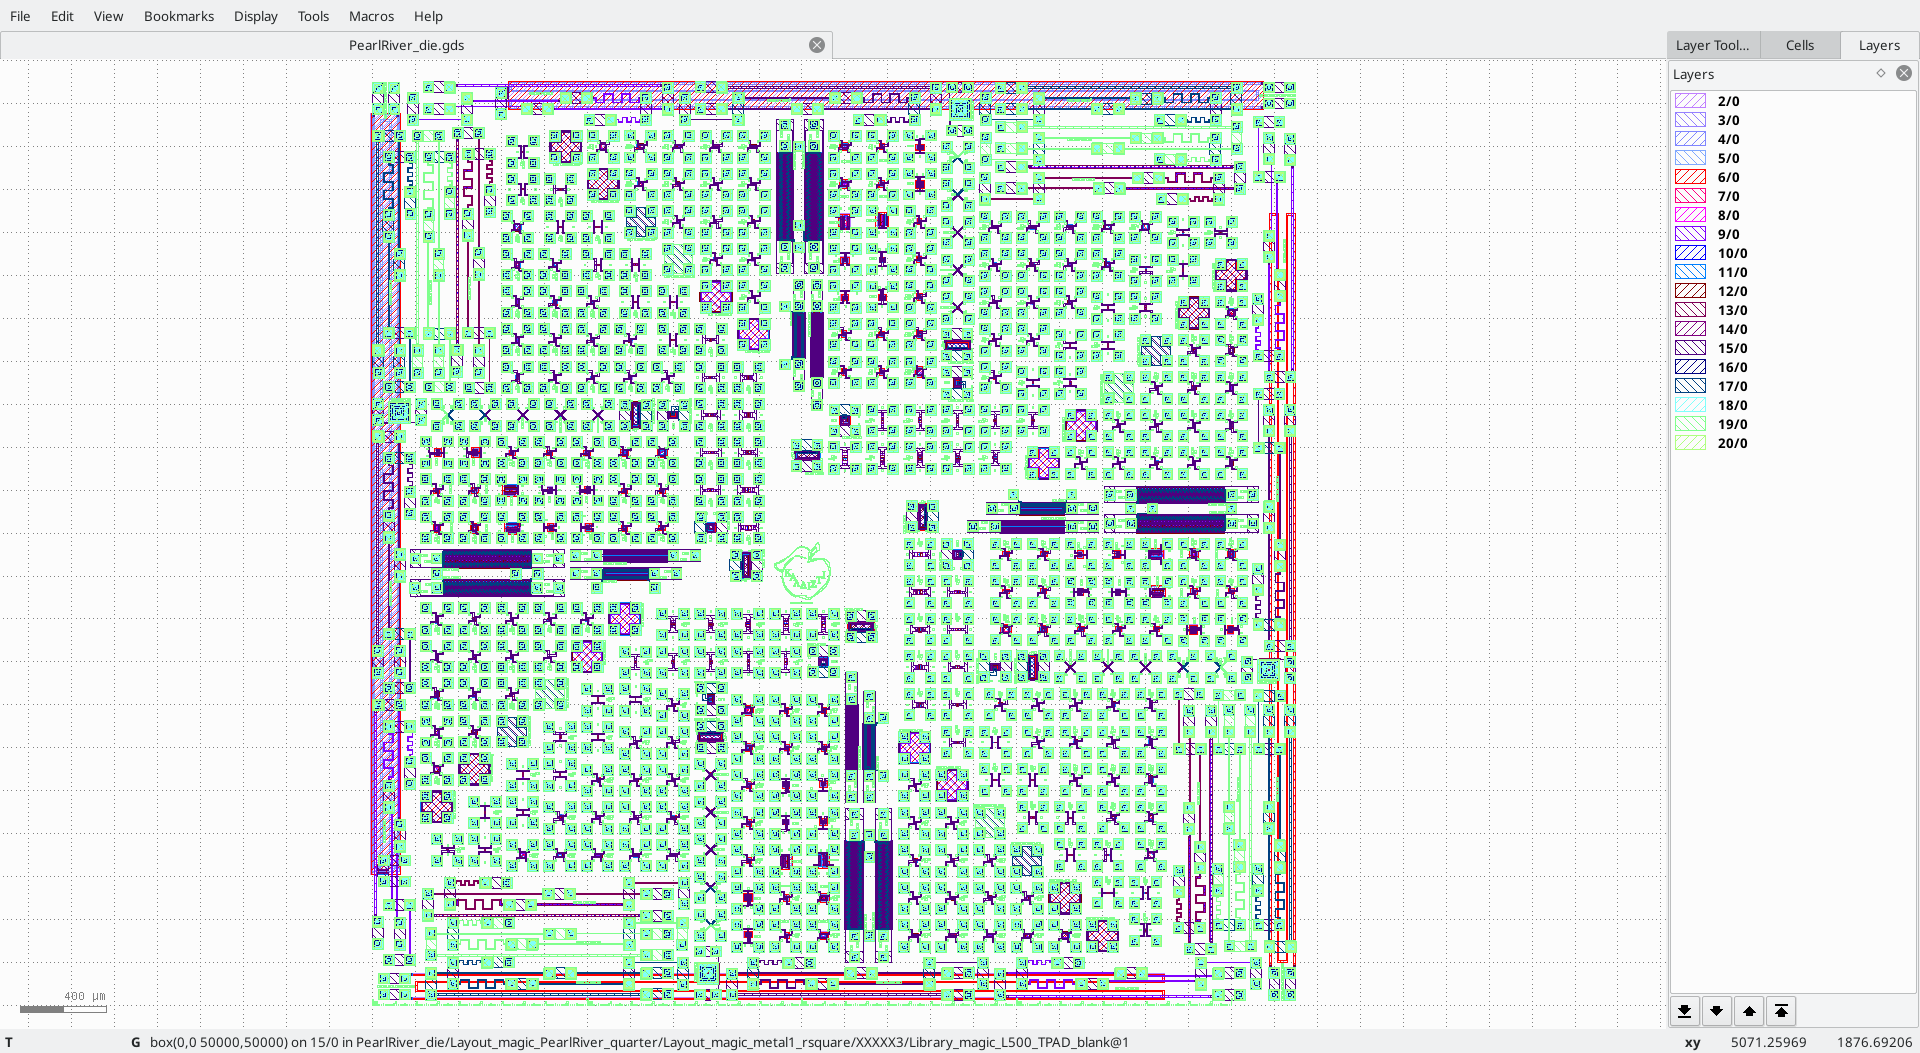
\includegraphics[height=0.8\textheight]{images/Screenshot_20181216_204924.png}
    \end{center}
\end{frame}

\begin{frame}{PearlRiver \cjkfont(珠江芯片一号)}
	\textbf{Fulfills following functions:}
	\begin{itemize}
		\item Debugging
		\item Calibration of new equipment to LibreSilicon
		\item Research of new features
		\item Syncing process features between fabs
	\end{itemize}
\end{frame}

\begin{frame}{Photomask}
\begin{center}
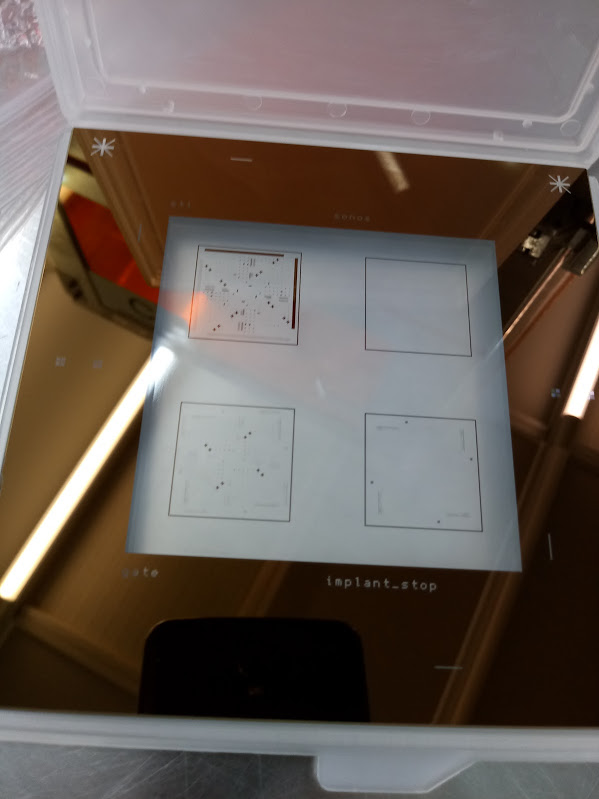
\includegraphics[height=0.8\textheight]{images/20181207_113845_Burst01.jpg}
\end{center}
\end{frame}

\begin{frame}{Photomask}
	\begin{itemize}
		\item Is stepper/aligner brand specific
		\item ASML stepper masks contain 4 layers each
		\item The NFF stepper has a reduction value of 5:1
		\item A 5 micron gate on the mask is 1 micron on the wafer
	\end{itemize}
\end{frame}

\begin{frame}{Photo resist (HKUST)}
\begin{center}
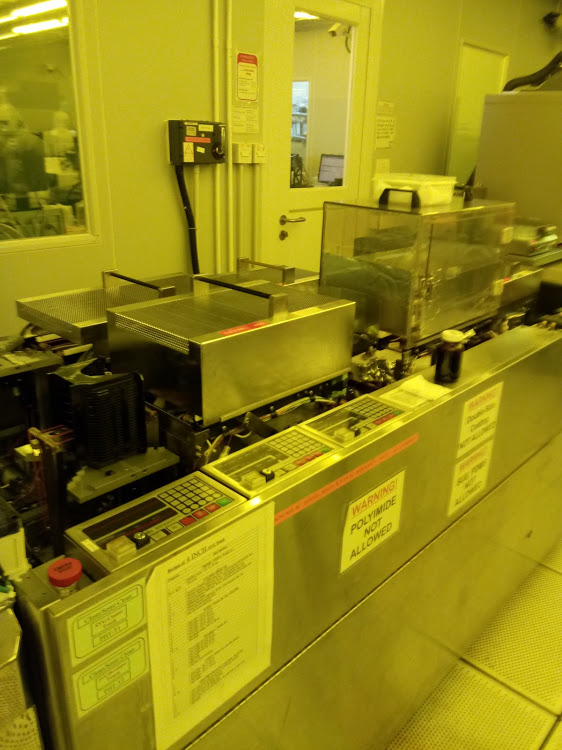
\includegraphics[height=0.8\textheight]{images/20181128_154907.jpg}
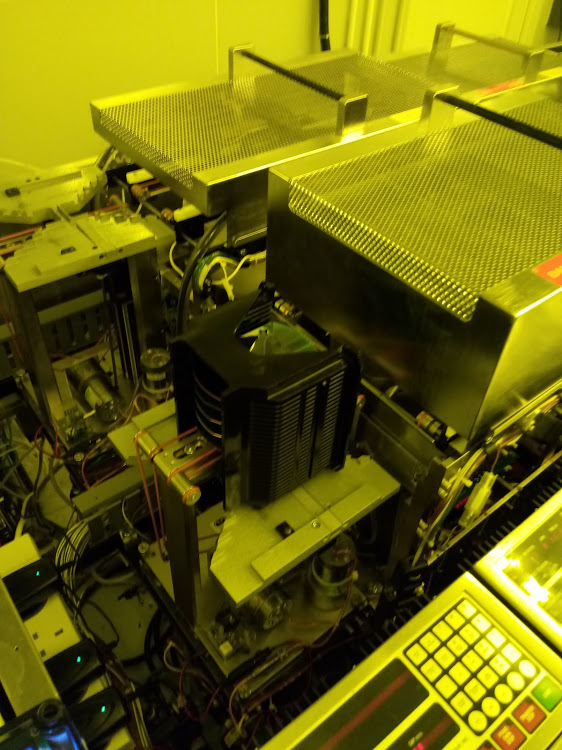
\includegraphics[height=0.8\textheight]{images/20181128_154911.jpg}
\end{center}
\end{frame}

\begin{frame}{Photo resist (HKUST)}
	\textbf{Two types of photo resist:}
	\begin{itemize}
		\item FH 6400L (implantation)
		\item HPR 504 (normal etch)
	\end{itemize}

	\textbf{Factors to consider:}
	\begin{itemize}
		\item Thickness of FH 6400L and implantation energy are interlinked
		\item Thickness of HPR 504 and etching time are interlinked (selectivity)
	\end{itemize}
\end{frame}

\begin{frame}{After exposure}
\begin{center}
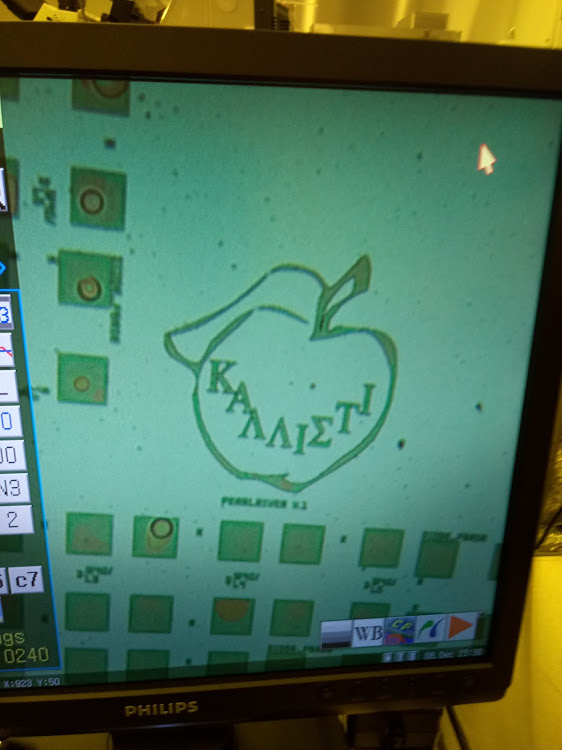
\includegraphics[height=0.8\textheight]{images/20181210_125830_Burst01.jpg}
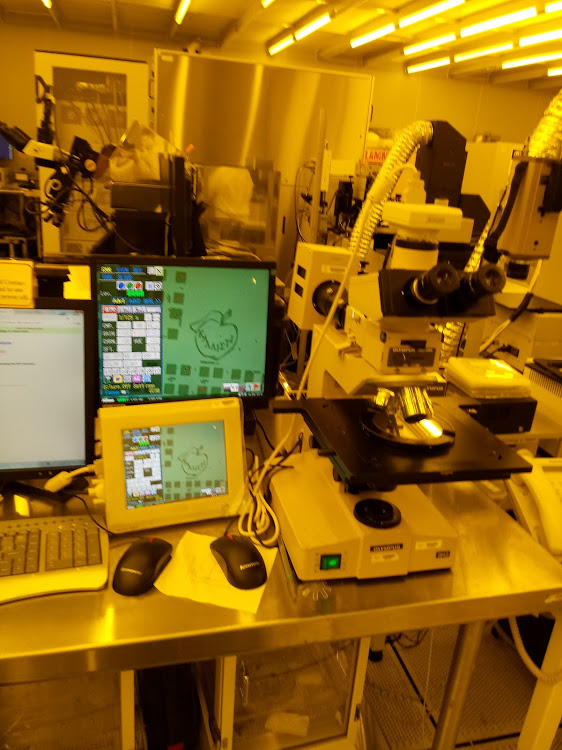
\includegraphics[height=0.8\textheight]{images/20181210_125845.jpg}
\end{center}
\end{frame}

\begin{frame}{Alignment}
\begin{center}
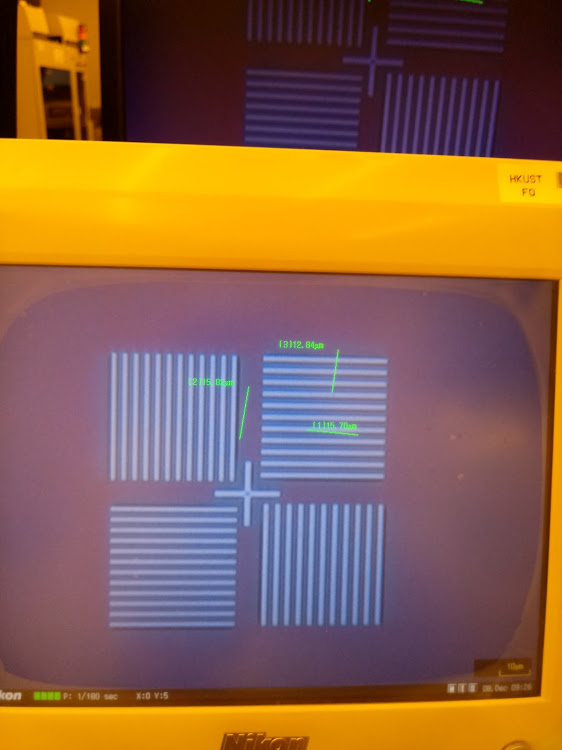
\includegraphics[height=0.8\textheight]{images/20181211_125918.jpg}
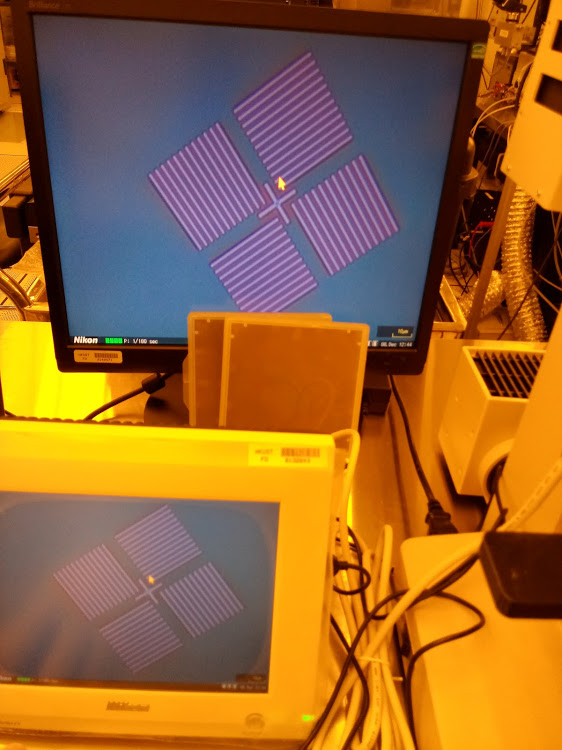
\includegraphics[height=0.8\textheight]{images/20181211_161801_Burst01.jpg}
\end{center}
\end{frame}

\begin{frame}{Example: NOR3 ring oscillator}
\begin{center}
	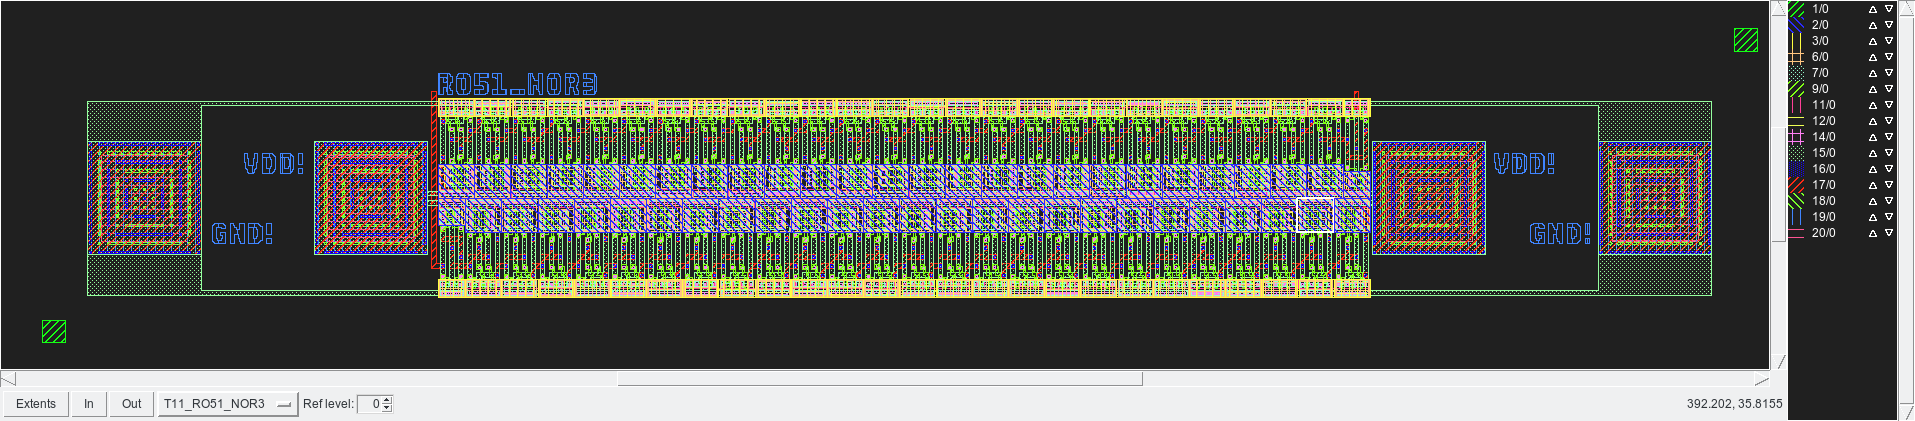
\includegraphics[width=\textwidth]{images/Screenshot_20181219_184458.png}
\end{center}
\end{frame}

\begin{frame}{Example: NOR3 ring oscillator}
\begin{center}
	\textbf{Metal interconnect (metal1):}

	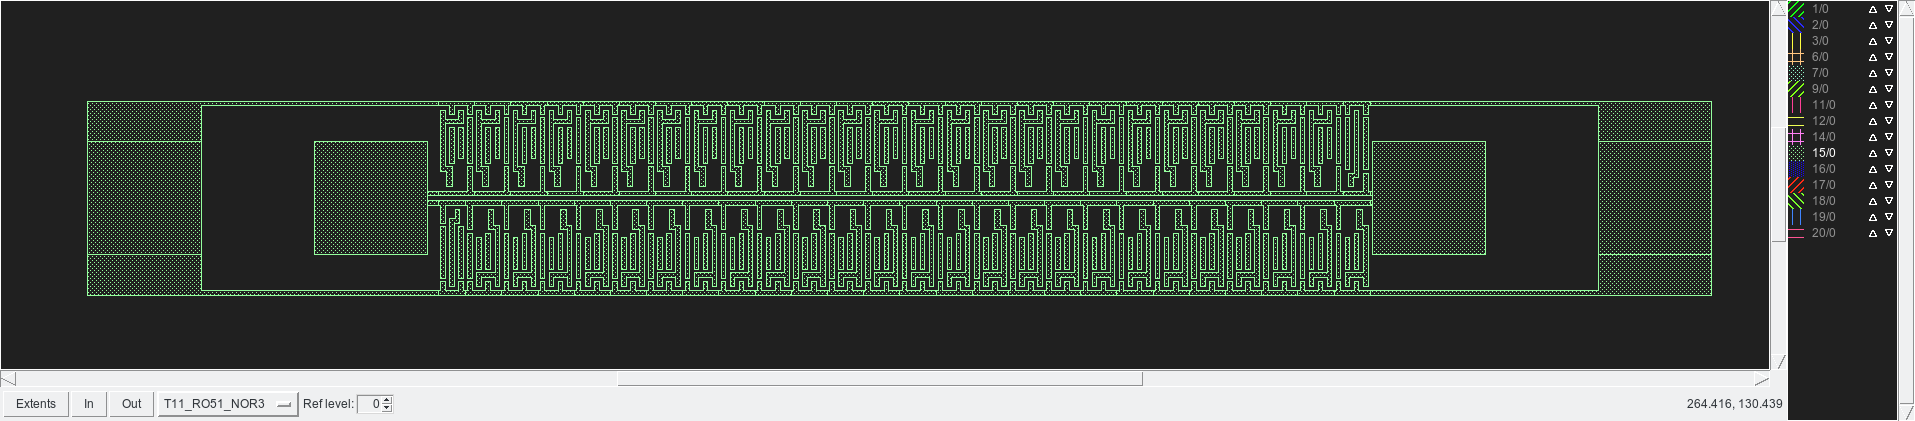
\includegraphics[width=\textwidth]{images/Screenshot_20181219_184526.png}
\end{center}
\end{frame}

\begin{frame}{Example: NOR3 ring oscillator}
\begin{center}
	\textbf{Metal interconnect (metal1):}

	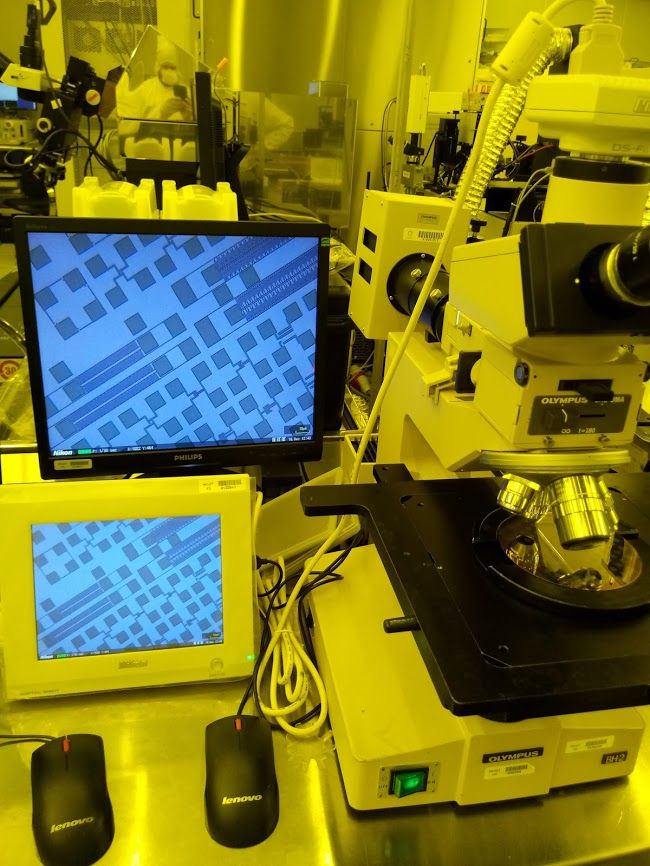
\includegraphics[width=0.25\textwidth]{images/20181218_115931.jpg}
	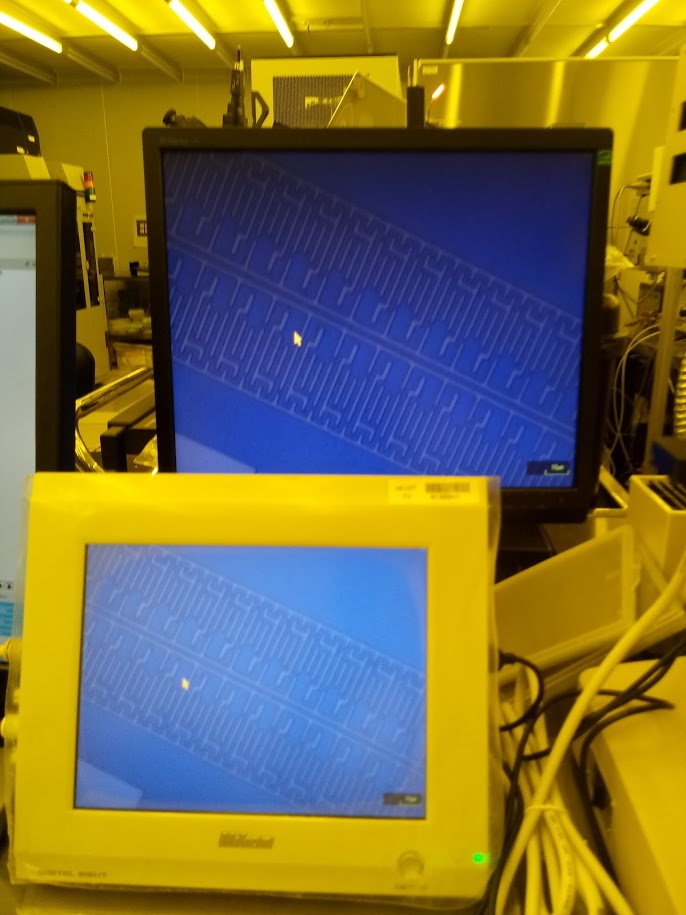
\includegraphics[width=0.25\textwidth]{images/20181218_161016.jpg}
\end{center}
\end{frame}

\begin{frame}{Example: NOR3 ring oscillator}
	\textbf{Recipe for metal interconnects:}

	\begin{itemize}
		\item Make a vacuum (low pressure)
		\item Deposit 100nm Aluminum
		\item Deposit 30nm Titanium over the Aluminum
		\item Take out of vacuum
		\item Dip into HF:DI (1:10) water solution for a few seconds until Titanium is gone
		\item Dip into FeCl3 or other suitable Aluminum etchant for around 30 seconds until Aluminum is gone
	\end{itemize}
	
\end{frame}


\begin{frame}{Example: NOR3 ring oscillator}
\begin{center}
	\textbf{Isolation (STI):}

	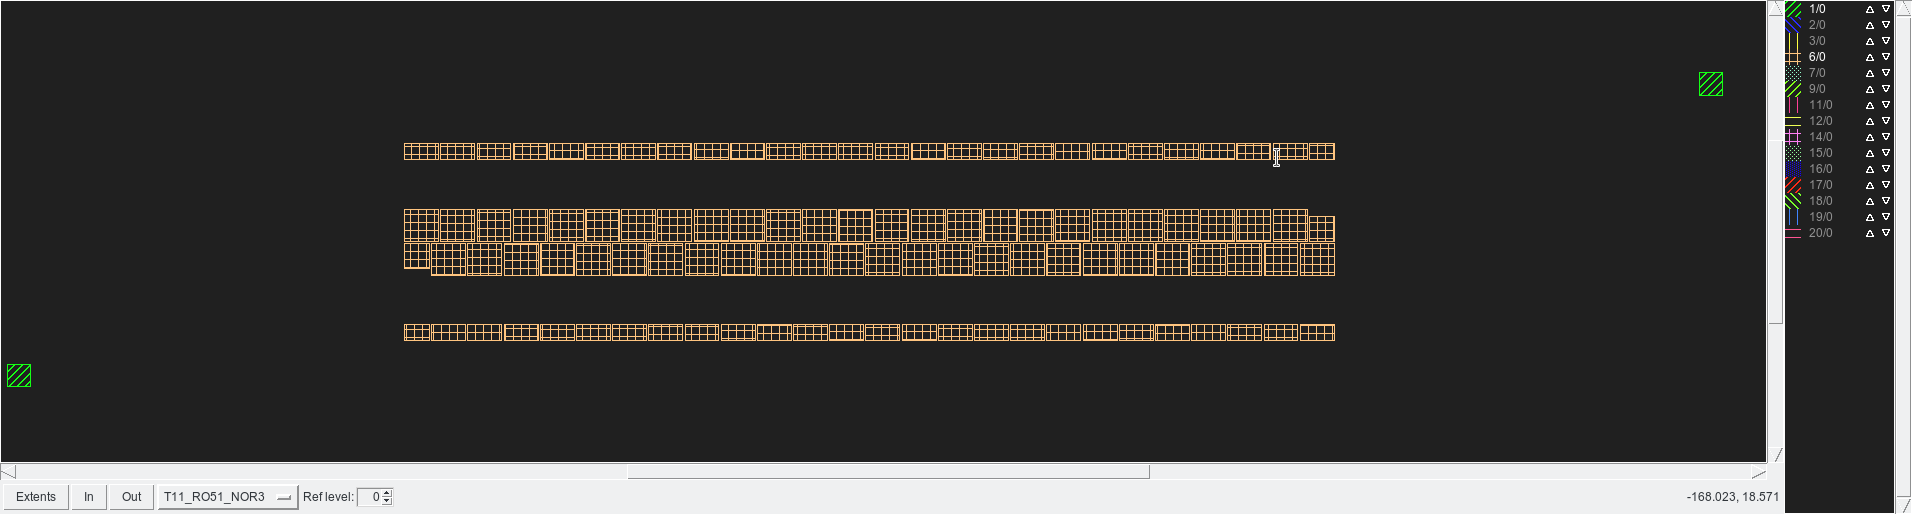
\includegraphics[width=\textwidth]{images/Screenshot_20181220_164222.png}
\end{center}
\end{frame}

\begin{frame}{Example: NOR3 ring oscillator}
\begin{center}
	\textbf{Isolation (STI):}

	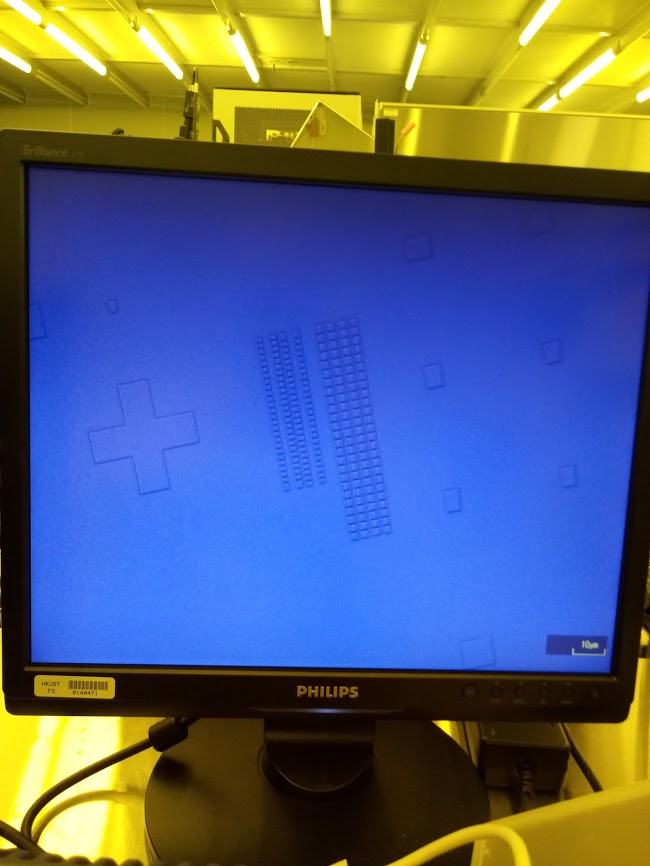
\includegraphics[width=0.25\textwidth]{images/20181219_125354_Burst01.jpg}
	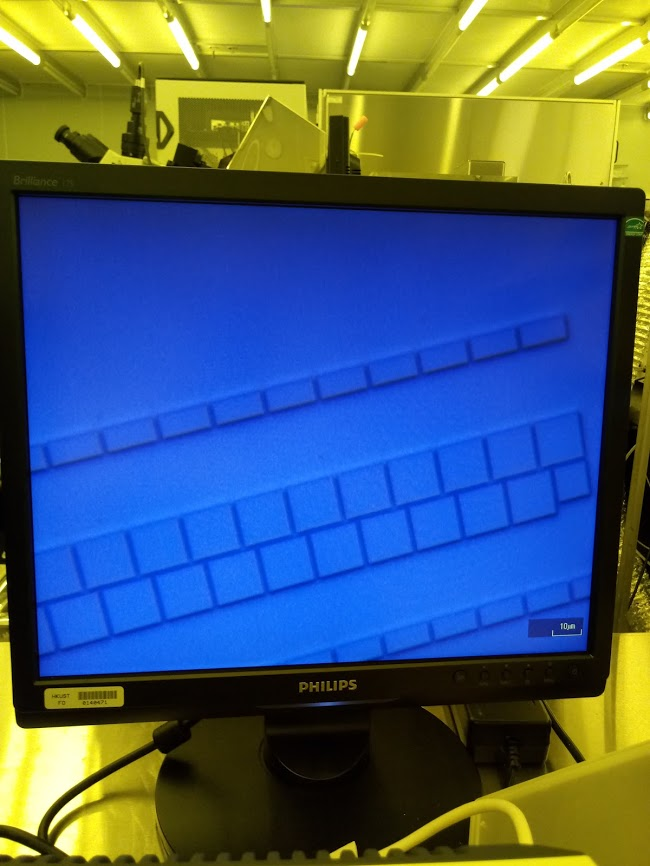
\includegraphics[width=0.25\textwidth]{images/20181219_125758.jpg}
\end{center}
\end{frame}

\begin{frame}{Example: NOR3 ring oscillator}
	\textbf{Recipe for STI:}
	\begin{itemize}
		\item\textbf{Dry}
		\begin{itemize}
			\item Plasma etching recipes are machine specific
			\item Variate the cycles for your recipe to match 2 microns
		\end{itemize}
		\item\textbf{Wet}
		\begin{itemize}
			\item Take TMAH: $ N ( CH _3 ) _4 ^{+} OH ^{−}$ (Tetramethylammonium hydroxide)
			\item Dilute with deionized water with DI:TMAH (3:1)
			\item Heat TMAH (25\%) to 80\textdegree{}C
			\item Dip wafer into the solution for around 6 minutes and 15 seconds (320nm/min, 2 microns)
		\end{itemize}
	\end{itemize}
\end{frame}
\end{document}
